% !TEX root = ../../defense.tex

\section{Geometric Control}

\subsection[Spacecraft Autonomy]{Spacecraft Autonomy}
% why study the coupled attitude/translational problem

\begin{frame}[t]{Spacecraft Autonomy} %-----------------------------%
\begin{itemize}
    \item Autonomous control of space vehicles is critical
    \begin{itemize}
        \item Avoid extensive planning and interaction by operators
        \item Ability to operate safely with system uncertainty 
        \item Independently navigate hazards and handle possible failures
    \end{itemize}
\end{itemize}
\visible<2>{
\begin{center}
    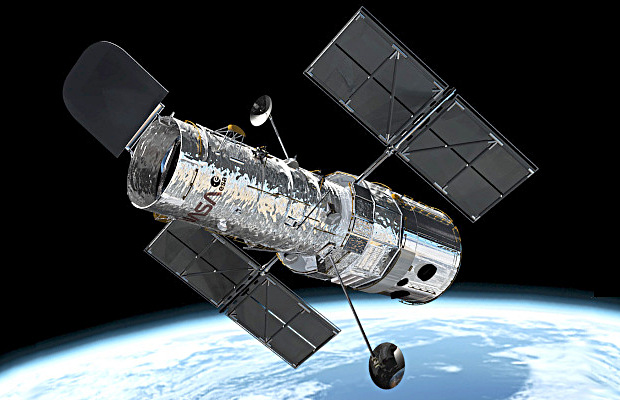
\includegraphics[width=0.5\textwidth,height=0.35\textheight,keepaspectratio]{figures/defense/hubble.jpg}\hfill
    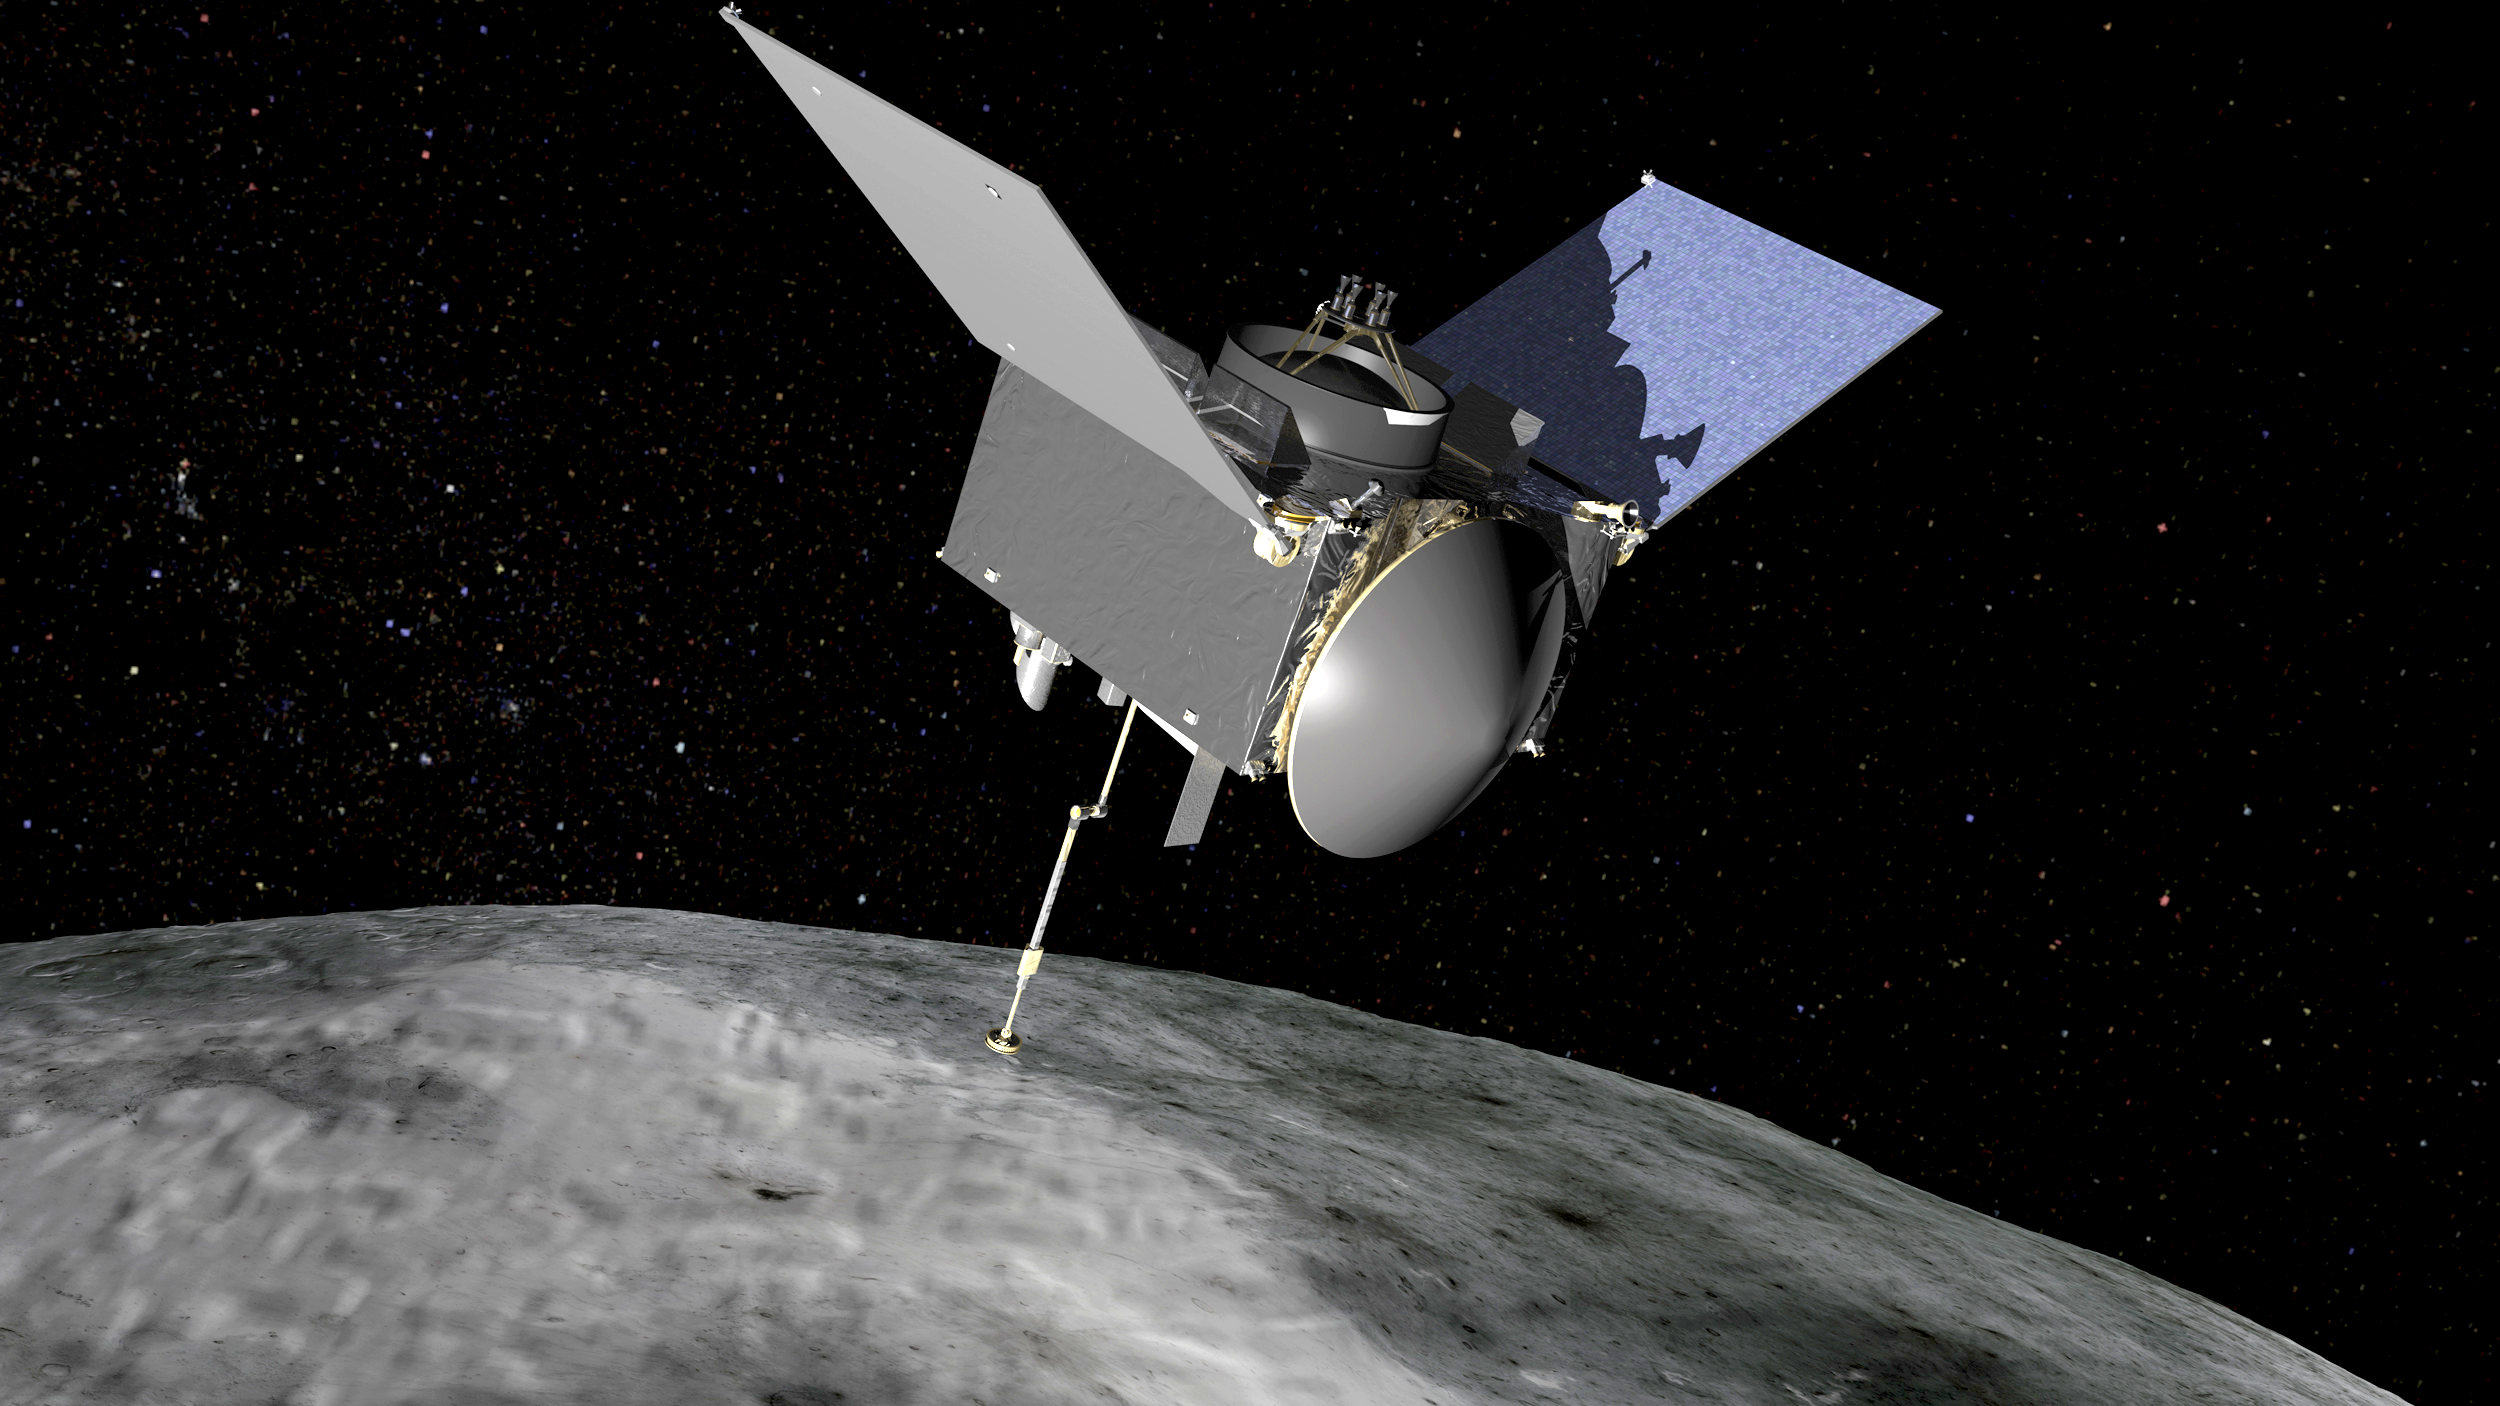
\includegraphics[width=0.5\textwidth,height=0.4\textheight,keepaspectratio]{figures/defense/osires_rex.png}
\end{center}
}
\note[itemize]{
    \item Autonomy is a key component to enable asteroid missions
}
\end{frame}   %-----------------------------%

\begin{frame}{Geometric Control}
Explain geometric control
\end{frame}

\subsection{Attitude Control}

\begin{frame}[t]{Problem Formulation} %-----------------------------------%
\begin{itemize}
    \item \Emph{Constrained attitude control} : reorient vehicle while avoiding pointing at obstacles
    \begin{itemize}
        \item Exclusion zones for payloads e.g infrared telescope
        \item UAVs manuevering in congested locations
        \item Laser/Radio emitters on spacecraft
    \end{itemize}
    \pause
    \item Previous approaches have several issues
    \begin{itemize}
        \item Attitude parameterizations: singularities/ambiguities
        \item Ad-hoc path planning: difficult to generalize to arbitrary obstacles
        \item Randomized methods: lack of stability guarantees
        \item Optimization based: expensive to compute and only provides open-loop control  
    \end{itemize}
\end{itemize}
\end{frame} %-------------------------------------%

\begin{frame}{Attitude Parameterizations}
    \begin{itemize}
        \item Euler Angles
        \begin{itemize}
            \item Minimal representation used for small attitude changes.
            \item Singularities exist for large angle slews: requires switching between 24 sequences
            \item Complicated trigonometric functions
        \end{itemize}
        \pause
        \item Quaternion 
        \begin{itemize}
            \item No singularities
            \item Two anti-podal quaternions for the same attitude
            \item Unwinding behavior for control systems
        \end{itemize}
        \pause
        \item Geometric control
        \begin{itemize}
            \item Globally and uniquely characterize attitude: \( R \in \SO \)
            \item Controller is globally valid for large angle maneuvers
        \end{itemize}
    \end{itemize}
    
\end{frame}

\begin{frame}{Objective} %---------------------------------------%

    \begin{block}{Nonlinear Control Design}
        Design control input \( u \) that stabilizes system from initial attitude \( R_0 \) to desired attitude \( R_d \) while avoiding obstacles
    \end{block}
    \pause
    \begin{itemize}
        \item Avoid drawbacks of other approaches 
        \begin{itemize}
            \item \Emph{Geometric control} - analysis is conducted directly on \( \SO \) 
            \item \Emph{Barrier function} - allows for arbitrary amount of constraints
            \item \Emph{Efficient } - real time feedback control
            \item \Emph{Stability} - Lyapunov analysis gives rigourous stability proof
            \item \Emph{Adaptive} - handles system uncertainties
        \end{itemize}
    \end{itemize}
\end{frame}


\begin{frame}{Spacecraft Orientation} %-----------------------------%

\begin{itemize}

    \item \Emph{Attitude Representation}: rotation matrix from body to inertial frame
     \[\SO =  \{R\in\R^{3\times 3}\,|\, R^TR=I,\;\mathrm{det}[R]=1\} . \]
    \item Rigid body attitude dynamics:
    \begin{gather*}
        J\dot\Omega + \Omega\times J\Omega = u+W(R,\Omega)\Delta , \quad \dot R = R\hat\Omega .
    \end{gather*}

    \item Sensor and obstacles defined by unit vectors in \( \R^3 \) 
        \begin{itemize}
            \item Body fixed sensor: \( r \in \S^2\)
            \item Inertially fixed hazard: \( v \in \S^2 \)
        \end{itemize} 
    \item Hard cone constraint: \( r^T R^T v \leq \cos \theta \)
    
\end{itemize}
\end{frame}   %-----------------------------%
